\documentclass{beamer}

% --- packages
\usepackage[utf8]{inputenc}
\usepackage[spanish]{babel}

\usepackage{bm}

\usepackage{nicematrix}

\usepackage{stanli}

\usepackage[style=apa,citestyle=apa]{biblatex}
% \DefineBibliographyStrings{spanish}{%
%   andothers = {et al}
%   }
\addbibresource{bibliografia.bib}
% ---

% --- tema
\usetheme{Madrid}
% ---

% --- Portada
\title[Cuaterniones en pyFEM] %optional
{Aplicación de los cuaterniones en el análisis matricial}

\subtitle{Implementación de pyFEM}

\author[Ramirez, Estrada] % (optional, for multiple authors)
{Cristian Ramirez \and Martín Estrada}

\institute[UNAL] % (optional)
{
  Facultad de ingeniería\\
  Universidad Nacional de Colombia
}

\date[INDETEC 2020] % (optional)
{IX seminario permanente de divulgación de resultados de investigación grupo INDETEC, Noviembre de 2020}

\logo{
\includegraphics[height=1.5cm]{escudo_unal.png}}
% ---

% --- contenido en cada sección
\AtBeginSection[]
{
  \begin{frame}
    \vfill
    \centering
    \begin{beamercolorbox}[sep=8pt,center,shadow=true,rounded=true]{title}
      \usebeamerfont{title}\secname\par%
    \end{beamercolorbox}
  \end{frame}
}
\AtBeginSubsection[]
{
  \begin{frame}
    \frametitle{Tabla de contenido}
    \tableofcontents[currentsubsection]
  \end{frame}
}
% ---

\begin{document}

\begin{frame}
  \titlepage
\end{frame}

% \section*{Outline}
\begin{frame}
  \frametitle{Tabla de contenido}
  \tableofcontents
\end{frame}

\section{Introducción}
\subsection{pyFEM}
\begin{frame}
  \frametitle{pyFEM y FEM.js}
  pyFEM: programa de computador para el análisis de estructuras en tres dimensiones tipo pórtico sometidas a cargas estáticas.
\end{frame}

\subsection{FEM.js}
\begin{frame}
  \frametitle{FEM.js}
  FEM.js: programa de computador para visualizar estructuras tridimensionales.
\end{frame}

\section{pyFEM}
\subsection{Elemento tipo pórtico}
\begin{frame}
  \frametitle{Elemento tipo pórtico}
  \begin{figure}
    \centering
    \begin{tikzpicture}[coords]
      % points
      \dpoint{a}{0}{0}{0};
      \dpoint{b}{4}{0}{0};

      \dpoint{alabel}{0}{0}{0.25};
      \dpoint{blabel}{4}{0}{0.25};

      \dpoint{beamlabel}{2}{0}{0.25};

      \dpoint{jux}{-1}{0}{0};
      \dpoint{juy}{0}{-1.5}{0.25};   
      \dpoint{juz}{0}{0}{-1.25};

      \dpoint{jrx}{-2}{0}{0};
      \dpoint{jry}{0}{-2.75}{0.25};   
      \dpoint{jrz}{0}{0}{-2.5};

      \dpoint{kux}{4.5}{0}{0};
      \dpoint{kuy}{4}{-1.5}{0.25};   
      \dpoint{kuz}{4}{0}{-1.25};

      \dpoint{krx}{5.25}{0}{0};
      \dpoint{kry}{4}{-2.75}{0.35};   
      \dpoint{krz}{4}{0}{-2.5};   
      
      % beams
      \dbeam{1}{a}{b};

      \dnotation{6}{beamlabel}{\emph{i}};

      % supports
      \dsupport{2}{a}[yz];
      \dsupport{2}{b}[yz];

      \dnotation{1}{alabel}{\emph{j}};
      \dnotation{1}{blabel}{\emph{k}};
      % restrains
      % j
      \dload{1}{a}[270][0][1];
      \dload{1}{a}[270][90][1][0.5];   
      \dload{1}{a}[180][180][1][0.5];

      \dload{3}{a}[270][0][1][1.25];
      \dload{3}{a}[270][90][1][1.75];   
      \dload{3}{a}[180][180][1][1.75];

      \dnotation{1}{jux}{1};
      \dnotation{1}{juy}{2};
      \dnotation{1}{juz}{3};

      \dnotation{1}{jrx}{4};
      \dnotation{1}{jry}{5};
      \dnotation{1}{jrz}{6};   
      
      % k
      \dload{2}{b}[90][0][1];
      \dload{1}{b}[270][90][1][0.5];   
      \dload{1}{b}[180][180][1][0.5];

      \dload{4}{b}[90][0][1][1.25];
      \dload{3}{b}[270][90][1][1.75];   
      \dload{3}{b}[180][180][1][1.75];

      \dnotation{1}{kux}{7};
      \dnotation{1}{kuy}{8};
      \dnotation{1}{kuz}{9};

      \dnotation{1}{krx}{10};
      \dnotation{1}{kry}{11};
      \dnotation{1}{krz}{12};
      
      % axes
      \dscaling{3}{1};
      \daxis{1}{0, 0, 0};
    \end{tikzpicture}
    \caption{Elemento tipo pórtico en coordenadas locales.}
    \label{fig:space-frame}
  \end{figure}
\end{frame}

\subsubsection{Matriz de rigidez}
\begin{frame}
  \frametitle{Matriz de rigidez}
  \begin{equation}
    \begin{bNiceArray}{CCCCCCCCCCCC}[small,
      first-row,
      first-col,
      code-for-first-row = \mathbf{\arabic{jCol}},
      code-for-first-col = \mathbf{\arabic{iRow}}
      ]
      
      & & & & & & & & & & & & \\
      & \frac{EA_x}{L} & 0 & 0 & 0 & 0 & 0 & -\frac{EA_x}{L} & 0 & 0 & 0 & 0 & 0 \\
      & & \frac{12EI_z}{L^3} & 0 & 0 & 0 & \frac{6EI_z}{L ^2} & 0 & -\frac{12EI_z}{L^3} & 0 & 0 & 0 & \frac{6EI_z}{L^2} \\
      & & & \frac{12EI_y}{L^3} & 0 & -\frac{6EI_y}{L^2} & 0 & 0 & 0 & -\frac{12EI_y}{L^3} & 0 & -\frac{6EI_y}{L^2} & 0 \\
      & & & & \frac{GI_x}{L} & 0 & 0 & 0 & 0 & 0 & -\frac{GI_x}{L} & 0 & 0 \\
      & & & & & \frac{4EI_y}{L} & 0 & 0 & 0 & \frac{6EI_y}{L^2} & 0 & \frac{2EI_y}{L} & 0 \\
      & & & & & & \frac{4EI_z}{L} & 0 & -\frac{6EI_z}{L^2} & 0 & 0 & 0 & \frac{2EI_z}{L} \\
      & & & & & & & \frac{EA_x}{L} & 0 & 0 & 0 & 0 & 0 \\
      & & & & & & & & \frac{12EI_z}{L^3} & 0 & 0 & 0 & -\frac{6EI_z}{L^2} \\
      & & & & & & & & & \frac{12EI_y}{L^3} & 0 & \frac{6EI_y}{L^2} & 0 \\
      & & & & & & & & & & \frac{GI_x}{L} & 0 & 0 \\
      & & & & & & & & & & & \frac{4EI_y}{L} & 0 \\
      & \text{sim.} & & & & & & & & & & & \frac{4EI_z}{L}
      \label{eq:matriz-rigidez-elemento-portico}
    \end{bNiceArray}
  \end{equation}
\end{frame}

\subsection{Teorema de rotación de Euler}
\begin{frame}
  \frametitle{Teorema de rotación de Euler}
  \begin{columns}
    \column{0.5\textwidth}
    \begin{block}{Definición}
      Según el \emph{teorema de rotación de Euler} (véase \cite{euler_rotations}), siempre es posible encontrar un diámetro de una esfera cuya posición es la misma después de rotarla alredor de su centro, por lo que cualquier secuencia de rotaciones de un sistema coordenado tridimensional es equivalente a una única rotación alrededor de un eje que pase por el origen.\\
    \end{block}

    \column{0.5\textwidth}
    \begin{figure}
      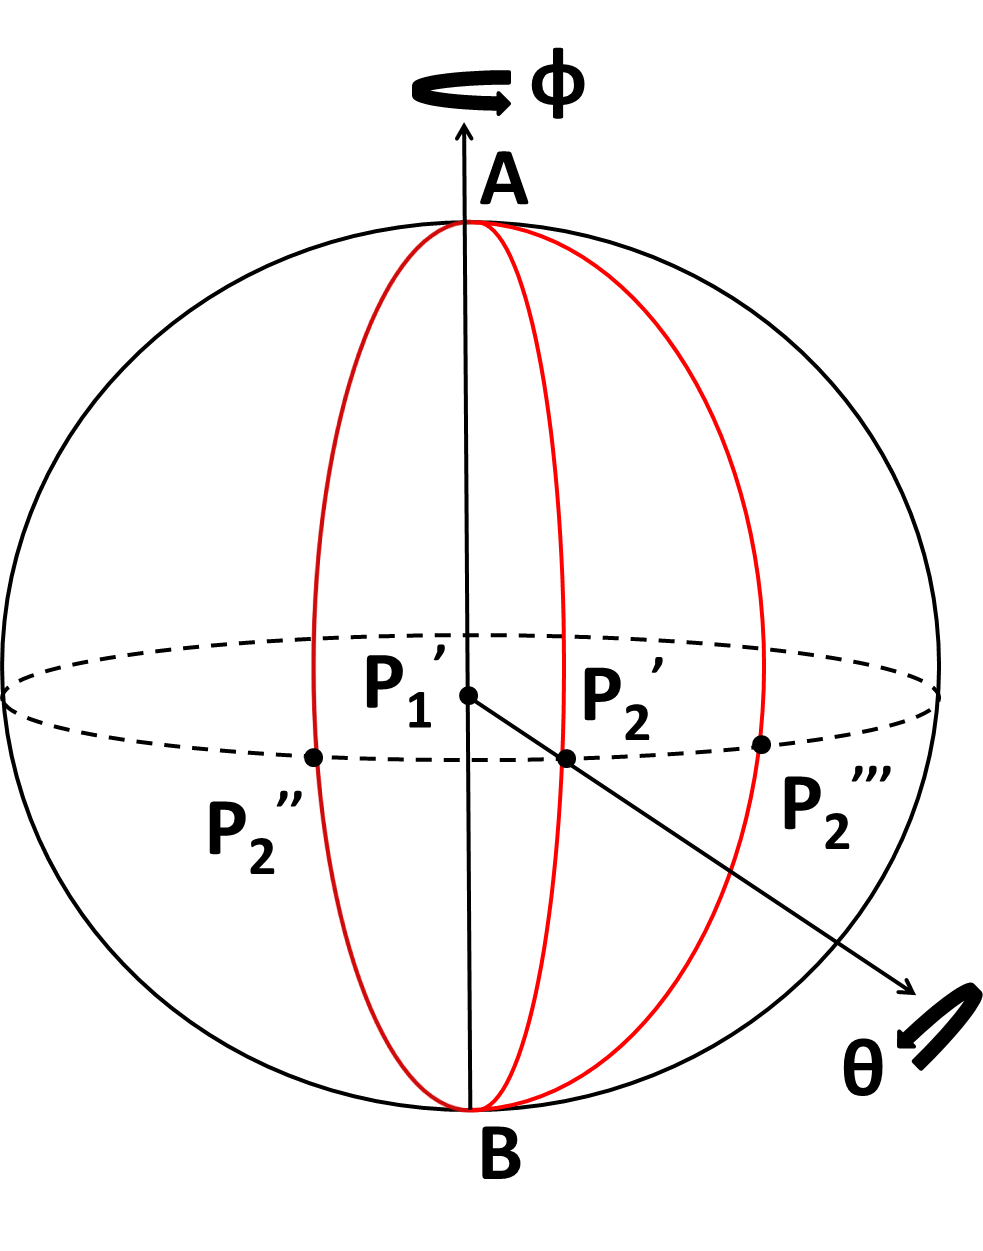
\includegraphics[width=0.5\textwidth]{euler_rotation.png}
    \end{figure}
  \end{columns}      
\end{frame}

\subsection{Rotación del sistema de coordenadas}
\begin{frame}
  \frametitle{Rotación del sistema de coordenadas}
  \begin{columns}
    \column{0.5\textwidth}
    El ángulo $ \theta $ y el vector $ n $  que definen la rotación del eje $ x $ del sistema de coordenadas global hacia el eje $ x_m $ del sistema de coordenadas de un elemento se puede calcular como
    \begin{equation}
      \begin{aligned}
        \mathbf{n} &= (1, 0, 0) \times \mathbf{x_m} \\
        \theta &= \arcsen((1, 0, 0) \cdot \mathbf{x_m})
      \end{aligned}
    \end{equation}
    \column{0.5\textwidth}
    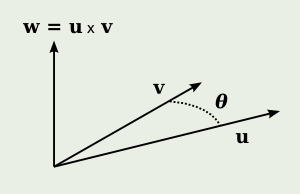
\includegraphics{quaternion_two_vectors.png}
  \end{columns}
\end{frame}

\subsection{Representación de la rotación como un cuaternión}
\begin{frame}
  \frametitle{Representación de la rotación como un cuaternión}
  Según \cite{dunn20023d}, la rotación de un sistema de coordenadas tridimensionales alrededor del eje $ \boldsymbol{n} $ una cantidad $ \boldsymbol{\theta} $ se puede describir mediante un \emph{cuaternión} como
  \begin{equation}
    \boldsymbol{q} =
    \begin{bmatrix}
      cos(\theta/2) & sin(\theta/2) \boldsymbol{n}
    \end{bmatrix} =
    \begin{bmatrix}
      w & x & y & z
    \end{bmatrix}
  \end{equation}
  y se puede obtener la matriz de rotación a partir de un cuaternión de la siguiente manera
  \begin{equation}
    \mathbf{R} =
    \begin{bNiceMatrix}
      1 - 2y^2-2z^2 & 2xy + 2wz & 2xz - 2wy \\
      2xy - 2wz & 1 - 2x^2-2z^2 & 2yz + 2wx \\
      2xz + 2wy & 2yz-2wx & 1 - 2x^2 - 2y^2
    \end{bNiceMatrix}
  \end{equation}
\end{frame}
\end{document}